\documentclass{article}
\usepackage{listings}
\usepackage{amsthm}
\usepackage{amsmath}
\usepackage{amssymb}
\usepackage{float}
\usepackage{url}
\usepackage{tikz}
\usepackage{tikz-cd}
\usepackage[utf8]{inputenc}

\ProvidesPackage{journal}
\usepackage{graphicx}
\usepackage{mathtools}
\usepackage{hyphenat}
\usepackage{hyperref}
\usepackage{adjustbox}
\usepackage{listings}
\usepackage{verbatim}
\usepackage{xcolor}
\usepackage{amsfonts}
\usepackage{amscd}
\usepackage{amsmath}
\usepackage{amssymb}
\usepackage{amsthm}
\usepackage{tikz}
\usepackage{tikz-cd}
\usepackage{url}
\usepackage[utf8]{inputenc}
\usepackage[english,ukrainian]{babel}
\usepackage{float}
\usepackage{url}
\usepackage{tikz}
\usepackage{tikz-cd}
\usepackage[utf8]{inputenc}
\usepackage{graphicx}
\usepackage[utf8]{inputenc}
\usepackage[T1]{fontenc}
\usepackage{lmodern}
\usepackage{tocloft}
\usepackage{hyperref}
\usepackage{xcolor}
\usepackage[only,llbracket,rrbracket,llparenthesis,rrparenthesis]{stmaryrd}

\usetikzlibrary{babel}

\newcommand*{\incmap}{\hookrightarrow}
\newcommand*{\thead}[1]{\multicolumn{1}{c}{\bfseries #1}}
\renewcommand{\Join}{\vee} % Join operation symbol
\newcommand{\tabstyle}[0]{\scriptsize\ttfamily\fontseries{l}\selectfont}

\lstset{
  basicstyle=\footnotesize,
  inputencoding=utf8,
  identifierstyle=,
  literate=
{𝟎}{{\ensuremath{\mathbf{0}}}}1
{𝟏}{{\ensuremath{\mathbf{1}}}}1
{≔}{{\ensuremath{\mathrm{:=}}}}1
{α}{{\ensuremath{\mathrm{\alpha}}}}1
{ᵂ}{{\ensuremath{^W}}}1
{β}{{\ensuremath{\mathrm{\beta}}}}1
{γ}{{\ensuremath{\mathrm{\gamma}}}}1
{δ}{{\ensuremath{\mathrm{\delta}}}}1
{ε}{{\ensuremath{\mathrm{\varepsilon}}}}1
{ζ}{{\ensuremath{\mathrm{\zeta}}}}1
{η}{{\ensuremath{\mathrm{\eta}}}}1
{θ}{{\ensuremath{\mathrm{\theta}}}}1
{ι}{{\ensuremath{\mathrm{\iota}}}}1
{κ}{{\ensuremath{\mathrm{\kappa}}}}1
{λ}{{\ensuremath{\mathrm{\lambda}}}}1
{μ}{{\ensuremath{\mathrm{\mu}}}}1
{ν}{{\ensuremath{\mathrm{\nu}}}}1
{ξ}{{\ensuremath{\mathrm{\xi}}}}1
{π}{{\ensuremath{\mathrm{\mathnormal{\pi}}}}}1
{ρ}{{\ensuremath{\mathrm{\rho}}}}1
{σ}{{\ensuremath{\mathrm{\sigma}}}}1
{τ}{{\ensuremath{\mathrm{\tau}}}}1
{φ}{{\ensuremath{\mathrm{\varphi}}}}1
{χ}{{\ensuremath{\mathrm{\chi}}}}1
{ψ}{{\ensuremath{\mathrm{\psi}}}}1
{ω}{{\ensuremath{\mathrm{\omega}}}}1
{Π}{{\ensuremath{\mathrm{\Pi}}}}1
{Γ}{{\ensuremath{\mathrm{\Gamma}}}}1
{Δ}{{\ensuremath{\mathrm{\Delta}}}}1
{Θ}{{\ensuremath{\mathrm{\Theta}}}}1
{Λ}{{\ensuremath{\mathrm{\Lambda}}}}1
{Σ}{{\ensuremath{\mathrm{\Sigma}}}}1
{Φ}{{\ensuremath{\mathrm{\Phi}}}}1
{Ξ}{{\ensuremath{\mathrm{\Xi}}}}1
{Ψ}{{\ensuremath{\mathrm{\Psi}}}}1
{Ω}{{\ensuremath{\mathrm{\Omega}}}}1
{ℵ}{{\ensuremath{\aleph}}}1
{≤}{{\ensuremath{\leq}}}1
{≥}{{\ensuremath{\geq}}}1
{≠}{{\ensuremath{\neq}}}1
{≈}{{\ensuremath{\approx}}}1
{≡}{{\ensuremath{\equiv}}}1
{≃}{{\ensuremath{\simeq}}}1
{≤}{{\ensuremath{\leq}}}1
{≥}{{\ensuremath{\geq}}}1
{∂}{{\ensuremath{\partial}}}1
{∆}{{\ensuremath{\triangle}}}1 % or \laplace?
{∫}{{\ensuremath{\int}}}1
{∑}{{\ensuremath{\mathrm{\Sigma}}}}1
{→}{{\ensuremath{\rightarrow}}}1
{⊥}{{\ensuremath{\perp}}}1
{∞}{{\ensuremath{\infty}}}1
{∂}{{\ensuremath{\partial}}}1
{∓}{{\ensuremath{\mp}}}1
{±}{{\ensuremath{\pm}}}1
{×}{{\ensuremath{\times}}}1
{⊕}{{\ensuremath{\oplus}}}1
{⊗}{{\ensuremath{\otimes}}}1
{⊞}{{\ensuremath{\boxplus}}}1
{∇}{{\ensuremath{\nabla}}}1
{√}{{\ensuremath{\sqrt}}}1
{⬝}{{\ensuremath{\cdot}}}1
{•}{{\ensuremath{\cdot}}}1
{∘}{{\ensuremath{\circ}}}1
{⁻}{{\ensuremath{^{-}}}}1
{▸}{{\ensuremath{\blacktriangleright}}}1
{★}{{\ensuremath{\star}}}1
{∧}{{\ensuremath{\wedge}}}1
{∨}{{\ensuremath{\vee}}}1
{¬}{{\ensuremath{\neg}}}1
{⊢}{{\ensuremath{\vdash}}}1
{⟨}{{\ensuremath{\langle}}}1
{⟩}{{\ensuremath{\rangle}}}1
{↦}{{\ensuremath{\mapsto}}}1
{→}{{\ensuremath{\rightarrow}}}1
{↔}{{\ensuremath{\leftrightarrow}}}1
{⇒}{{\ensuremath{\Rightarrow}}}1
{⟹}{{\ensuremath{\Longrightarrow}}}1
{⇐}{{\ensuremath{\Leftarrow}}}1
{⟸}{{\ensuremath{\Longleftarrow}}}1
{∩}{{\ensuremath{\cap}}}1
{∪}{{\ensuremath{\cup}}}1
{·}{{\ensuremath{\cdot}}}1
{ᵢ}{{\ensuremath{_i}}}1
{ⱼ}{{\ensuremath{_j}}}1
{₊}{{\ensuremath{_+}}}1
{ℑ}{{\ensuremath{\Im}}}1
{𝒢}{{\ensuremath{\mathcal{G}}}}1
{ℕ}{{\ensuremath{\mathbb{N}}}}1
{𝟘}{{\ensuremath{\mathbb{0}}}}1
{ℤ}{{\ensuremath{\mathbb{Z}}}}1
{ℝ}{{\ensuremath{\mathbb{R}}}}1
{⊂}{{\ensuremath{\subseteq}}}1
{⊆}{{\ensuremath{\subseteq}}}1
{⊄}{{\ensuremath{\nsubseteq}}}1
{⊈}{{\ensuremath{\nsubseteq}}}1
{⊃}{{\ensuremath{\supseteq}}}1
{⊇}{{\ensuremath{\supseteq}}}1
{⊅}{{\ensuremath{\nsupseteq}}}1
{⊉}{{\ensuremath{\nsupseteq}}}1
{∈}{{\ensuremath{\in}}}1
{∉}{{\ensuremath{\notin}}}1
{∋}{{\ensuremath{\ni}}}1
{∌}{{\ensuremath{\notni}}}1
{∅}{{\ensuremath{\emptyset}}}1
{∖}{{\ensuremath{\setminus}}}1
{†}{{\ensuremath{\dag}}}1
{ℕ}{{\ensuremath{\mathbb{N}}}}1
{ℤ}{{\ensuremath{\mathbb{Z}}}}1
{ℝ}{{\ensuremath{\mathbb{R}}}}1
{ℚ}{{\ensuremath{\mathbb{Q}}}}1
{ℂ}{{\ensuremath{\mathbb{C}}}}1
{⌞}{{\ensuremath{\llcorner}}}1
{⌟}{{\ensuremath{\lrcorner}}}1
{⦃}{{\ensuremath{ \{\!| }}}1
{⦄}{{\ensuremath{ |\!\} }}}1
{ᵁ}{{\ensuremath{^U}}}1
{₋}{{\ensuremath{_{-}}}}1
{₁}{{\ensuremath{_1}}}1
{₂}{{\ensuremath{_2}}}1
{₃}{{\ensuremath{_3}}}1
{₄}{{\ensuremath{_4}}}1
{₅}{{\ensuremath{_5}}}1
{₆}{{\ensuremath{_6}}}1
{₇}{{\ensuremath{_7}}}1
{₈}{{\ensuremath{_8}}}1
{₉}{{\ensuremath{_9}}}1
{₀}{{\ensuremath{_0}}}1
{¹}{{\ensuremath{^1}}}1
{ₙ}{{\ensuremath{_n}}}1
{ₘ}{{\ensuremath{_m}}}1
{↑}{{\ensuremath{\uparrow}}}1
{↓}{{\ensuremath{\downarrow}}}1
{▸}{{\ensuremath{\triangleright}}}1
{∀}{{\ensuremath{\forall}}}1
{∃}{{\ensuremath{\exists}}}1
{λ}{{\ensuremath{\mathrm{\lambda}}}}1
{=}{{\ensuremath{=}}}1
{<}{{\ensuremath{\textless}}}1
{>}{{\ensuremath{\textgreater}}}1
{_}{{$\_$}}1
{(}{(}1
{(}{(}1
{‖}{{\ensuremath{\Vert}}}1
{+}{{+}}1
{*}{{*}}1,
}

\theoremstyle{definition}
\newtheorem{definition}{Definition}
\newtheorem{theorem}{Theorem}
\newtheorem{lemma}{Lemma}
\newtheorem{example}{Example}



\begin{document}

\title{Issue III: Homotopy Type Theory}
\author{Maksym Sokhatskyi $^1$}
\date{ $^1$ National Technical University of Ukraine \\
       \small Igor Sikorsky Kyiv Polytechnical Institute \\
       \today }

\maketitle

\begin{abstract}
Here is presented destinctive points of Homotopy Type Theory
as an extension of Martin-Löf Type Theory but without higher inductive types
which will be given in the next issue. The study of identity system is given.
Groupoid (categorical) interpretation is presented as categories of spaces and paths between them as invertible morphisms.
At last constructive proof $\Omega(S^1)=\mathbb{Z}$ is given through helix.
\\
\\
{\bf Keywords}: Homotopy Theory, Type Theory
\end{abstract}

\ifincludeTOC
  \tableofcontents
\else
  \addtocontents{toc}{\protect\newpage}
\fi

\newpage
\section{Groupoid Interpretation}
\subsection{Introduction: Type Theory}
Type theory is a universal programming language for pure mathematics,
designed for theorem proving. It supports an arbitrary number of consistent
axioms, structured as pseudo-isomorphisms consisting of \textit{encode}
functions (methods for constructing type elements), \textit{decode}
functions (dependent eliminators of the universal induction principle),
and their equations---beta and eta rules governing computability and
uniqueness.

As a programming language, type theory includes basic
primitives (axioms as built-in types) and accompanying documentation,
such as lecture notes or textbooks, explaining their applications, including:

\begin{itemize}
\item \text{Function} ($\mathbf{\Pi}$)
\item \text{Context} ($\mathbf{\Sigma}$)
\item \text{Identification} ($\mathbf{=}$)
\item \text{Polynomial} ($\mathbf{W}$)
\item \text{Path} ($\Xi$)
\item \text{Gluing} ($\mathbf{Glue}$)
\item \text{Infinitesimal} ($\Im$)
\item \text{Complex} ($\mathbf{HIT}$)
\end{itemize}

Students (10) are tasked with applying type theory to prove an initial
but non-trivial result addressing an open problem in one of the following
areas offered by the Department of Pure Mathematics (KM-111):

\[
\text{Mathematics} :=
\begin{cases}
\text{Homotopy Theory} \\
\text{Homological Algebra} \\
\text{Category Theory} \\
\text{Functional Analysis} \\
\text{Differential Geometry}
\end{cases} .
\]


\newpage
\subsection{Motivation: Homotopy Type Theory}
The primary motivation of homotopy type theory is to provide computational
semantics for homotopic types and CW-complexes. The central idea, as
described in, is to combine function spaces (\(\Pi\)),
context spaces (\(\Sigma\)), and path spaces (\(\Xi\)) to form a fiber bundle, proven within HoTT to coincide with the $\Pi$ type itself.

Key definitions include:

\begin{lstlisting}
def contr (A: U) : U := Σ (x: A), Π (y: A), Ξ A x y
def fiber (A B: U) (f: A → B) (y: B): U := Σ (x: A), Path B y (f x)
def isEquiv (A B: U) (f: A → B): U := Π (y: B), contr(fiber A B f y)
def equiv (X Y: U): U := Σ (f: X → Y), isEquiv X Y f
def ua (A B : U) (p : Ξ U A B) : equiv A B
 := transp (<i> equiv A (p @ i)) 0 (idEquiv A)
\end{lstlisting}

The absence of an eta-rule for equality implies that not all proofs of the
same path space are equal, resulting in a multidimensional \(\infty\)-groupoid
structure for path spaces. Further definitions include:

\begin{lstlisting}
def isProp (A : U) : U
 := Π (a b : A), Ξ A a b

def isSet (A : U) : U
 := Π (a b : A) (x y : Ξ A a b), Ξ (Ξ A a b) x y

def isGroupoid (A : U) : U
 := Π (a b : A) (x y : Ξ A a b) (i j : Ξ (Ξ A a b) x y),
    Ξ (Ξ (Ξ A a b) x y) i j
\end{lstlisting}

The groupoid interpretation raises questions about the existence of a language for
mechanically proving all properties of the categorical definition of a groupoid:

\begin{lstlisting}
def CatGroupoid (X : U) (G : isGroupoid X)
  : isCatGroupoid (PathCat X)
 := ( idp X,
      comp-Path X,
      G,
      sym X,
      comp-inv-Path⁻¹ X,
      comp-inv-Path X,
      comp-Path-left X,
      comp-Path-right X,
      comp-Path-assoc X,
      ★
    )
\end{lstlisting}

\newpage
\subsection{Metatheory: Adjunction Triples}
The course is divided into four parts, each exploring type-axioms and their meta-theoretical adjunctions.

\subsubsection{Fibrational Proofs}
\[
\Sigma \dashv f_\star \dashv \Pi
\]
Fibrational proofs are modeled by primitive axioms, which are type-theoretic
representations of categorical meta-theoretical models of adjunctions of three
Cockett-Reit functors, giving rise to function spaces (\(\Pi\)) and pair
spaces (\(\Sigma\)). These proof methods enable direct analysis of fibrations.

\subsubsection{Equality Proofs}
\[
\mathrm{Q} \dashv \Xi \dashv \mathrm{C}
\]
In intensional type theory, the equality type is embedded as type-theoretic
primitives of categorical meta-theoretical models of adjunctions of three
Jacobs-Lambek functors: quotient space (\(\mathrm{Q}\)), identification
system (\(\Xi\)), and contractible space (\(\mathrm{C}\)). These methods allow
direct manipulation of identification systems, strict for set theory and
homotopic for homotopy theory.

\subsubsection{Inductive Proofs}
$$
\mathrm{W} \dashv \odot \dashv \mathrm{M}
$$

Inductive types in type theory can be embedded as polynomial
functors ($\mathrm{W}$, $\mathrm{M}$) or general inductive type
schemes (Calculus of Inductive Constructions), with properties including:
1) Verification of program finiteness;
2) Verification of strict positivity of parameters;
3) Verification of mutual recursion.

In this course, induction and coinduction are introduced as type-theoretic
primitives of categorical meta-theoretical models of adjunctions of
polynomial functors (Lambek-Bohm), enabling manipulation of initial
and terminal algebras, algebraic recursive data types, and infinite
processes. Higher inductive proofs, where constructors include path
spaces, are modeled by polynomial functors using monad-algebras and
comonad-coalgebras (Lumsdaine-Shulman).

\subsection*{Historical Notes}
Homotypy Type Theory takes its origins in 1996 from groupoid interpretation by
Hofmann and Streicher's, and later (in 10 years) was formalized by Awodey,
Warren and Voevodsky. Voevodsky constrtucted Kan simplicial sets interpretation
of type theory and discovered the property of this model, that was named univalence.
This property allows to identify isomorphic structures in terms of type theory.

Homotopy type theory to classical homotopy theory is like Euclidian
syntethic geometry (points, lines, axioms and deduction rules) to
analytical geometry with cartesian coordinates on $\mathbb{R}^n$ (geometric and algebraic)\footnote{We will denote geometric, type theoretical and homotopy constants
bold font $\mathbf{R}$ while analitical will be denoted with double lined letters $\mathbb{R}$.}.

In the same way as inductive types extends MLTT for inductive programming,
the higher inductive types (HIT) extend homotopy type theory for geometry programming.
You can directly encode CW-complexes by using HIT. The definition of HIT syntax will
be given in the next {\bf Issue IV: Higher Inductive Types}.

Cubical with HITs has very lightweight core and syntax, and
is an internal language of $(\infty,1)$-topos.
Cubical with $[0,1]$ Path types but without HITs is an
internal language of $(\infty,1)$-categories, while MLTT
is an internal language of locally cartesian closed categories.

\subsection*{Acknowledgement}
This article is dedicated to Ihor Horobets and written on his
request for clarification and direct intoduction to HoTT.

\newpage
\section{Homotopy Type Theory}

\subsection{Identity Systems}
\begin{definition} (Identity System).
An identity system over type $A$ in universe $X_i$ is a
family $R : A \rightarrow A \rightarrow X_i$ with a function
$r_0: \Pi_{a:A}R(a,a)$ such that any type family
$D : \Pi_{a,b:A}R(a,b) \rightarrow X_i$ and
$d: \Pi_{a:A}D(a,a,r_0(a))$, there exists a function
$f: \Pi_{a,b:A}\Pi_{r:R(a,b)}D(a,b,r)$ such that
$f(a,a,r_0(a))=d(a)$ for all $a:A$.
\begin{lstlisting}
def IdentitySystem (A : U) : U
 := Σ (=-form : A → A → U)
      (=-ctor : Π (a : A), =-form a a)
      (=-elim : Π (a : A) (C: Π (x y : A)
                  (p : =-form x y), U)
                  (d : C a a (=-ctor a)) (y : A)
                  (p : =-form a y), C a y p)
      (=-comp : Π (a : A) (C: Π (x y : A)
                  (p : =-form x y), U)
                  (d : C a a (=-ctor a)),
                  Ξ (C a a (=-ctor a)) d
                       (=-elim a C d a (=-ctor a))), 𝟏
\end{lstlisting}
\end{definition}

\begin{example}
There are number of equality signs used in this tutorial,
all of them listed in the following table of identity systems:
$$
\begin{array}{ll} \mathrm{Sign} & \mathrm{Meaning} \\
                         \hline
                        =_{def} & \mathrm{Definition} \\
                              = & \mathrm{Id} \\
                         \equiv & \mathrm{Path} \\
                         \simeq & \mathrm{Equivalence} \\
                          \cong & \mathrm{Isomorphism} \\
                           \sim & \mathrm{Homotopy} \\
                        \approx & \mathrm{Bisimulation} \\
                      \end{array}
$$
\end{example}

\begin{theorem} (Fundamental Theorem of Identity System).
\end{theorem}

\begin{definition} (Strict Identity System).
An identity system over type $A$ and universe
of pretypes $V_i$ is called strict identity system ($=$), which respects UIP.
\end{definition}

\begin{definition} (Homotopy Identity System).
An identity system over type $A$ and universe of homotopy
types $U_i$ is called homotopy identity system ($\equiv$),
which models discrete infinity groupoid.
\end{definition}

\newpage
\subsection{Path ($\Xi$)}
The homotopy identity system defines a $\mathbf{Path}$
space indexed over type $A$
with elements as functions from interval $[0,1]$ to values
of that path space $[0,1] \rightarrow A$. HoTT book
defines two induction principles for identity types:
path induction and based path induction.

\begin{definition} (Path Formation).
$$
  \equiv\hspace{0.4em}: U =_{def} \prod_{A:U}\prod_{x,y:A} \mathbf{Path}_A(x,y).
$$
\begin{lstlisting}[mathescape=true]
def Ξ (A : U) (x y : A) : U
 := PathP (<_> A) x y

def $\Xi'$ (A : U) (x y : A)
 := Π (i : I),
    A [∂ i |-> [(i = 0) → x ,
                (i = 1) → y ]]
\end{lstlisting}
\end{definition}

\begin{definition} (Path Introduction).
Returns a reflexivity path space for a given value of the type.
The inhabitant of that path space is the lambda on the homotopy
interval $[0,1]$ that returns a constant value $x$. Written in
syntax as $[i]x$.
$$
  \mathrm{id_\equiv} : x \equiv_A x =_{def} \prod_{A:U}\prod_{x:A} [i] x
$$
\begin{lstlisting}[mathescape=true]
def idp (A: U) (x: A)
  : Ξ A x x := <_> x
\end{lstlisting}
\end{definition}

\begin{definition} (Path Application).
\begin{lstlisting}[mathescape=true]
def at0 (A: U) (a b: A)
    (p: Path A a b) : A := p @ 0

def at1 (A: U) (a b: A)
    (p: Path A a b): A := p @ 1
\end{lstlisting}
\end{definition}

\newpage

\begin{definition} (Path Connections).
Connections allow you to build a square
with only one element of path: i) $[i,j] p\ @\ min(i,j)$;
ii) $[i,j] p\ @\ max(i,j)$.

\[
\begin{array}{cc}
  \begin{tikzcd}
    b \arrow[r, "{[i]b}"] & b \\
    a \arrow[u, "p"] \arrow[r, "p"] & b \arrow[u, "{[i]b}"]
  \end{tikzcd}
  \begin{tikzcd}
    a \arrow[r, "p"] & b \\
    a \arrow[u, "{[i]a}"] \arrow[r, "{[i]a}"] & a \arrow[u, "p"]
  \end{tikzcd}
\end{array}
\]

\begin{lstlisting}[mathescape=true]
def join (A: U) (a b: A) (p: Path A a b)
  : PathP (<x> Path A (p@x) b) p (<i> b)
 := <y x> p @ (x \/ y)

def meet (A: U) (a b: A) (p: Path A a b)
  : PathP (<x> Path A a (p@x)) (<i> a) p
 := <x y> p @ (x /\ y)
\end{lstlisting}
\end{definition}

\begin{definition} (Path Inversion).
\end{definition}

\begin{theorem} (Congruence).
$$
\mathrm{ap} : f(a)\equiv f(b) =_{def}
$$
$$
  \prod_{A:U}\prod_{a,x:A}\prod_{B:A\rightarrow U}\prod_{f: \Pi(A,B)}\prod_{p:a\equiv_A x}[i] f(p@i).
$$
\begin{lstlisting}[mathescape=true]
def ap (A B: U) (f: A -> B)
    (a b: A) (p: Path A a b)
  : Path B (f a) (f b)

def apd (A: U) (a x: A) (B: A -> U)
    (f: A -> B a) (b: B a) (p: Path A a x)
  : Path (B a) (f a) (f x)
\end{lstlisting}
\end{theorem}

Maps a given path space between values of one type
to path space of another type using an encode function between types.
Implemented as a lambda defined on $[0,1]$ that returns
application of encode function to path application of
the given path to lamda argument $[i]f (p @ i)$
in both cases.

\newpage

\begin{definition} (Generalized Transport Kan Operation).
Transports a value of the left type to the value of the right type
by a given path element of the path space between left and right types.
$$
  \mathrm{transport} : A(0) \rightarrow A(1) =_{def}
$$
$$
  \prod_{A:I\rightarrow U}\prod_{r:I}
$$
$$
  \lambda x,\mathbf{transp}([i]A(i),0,x).
$$
\begin{lstlisting}[mathescape=true]
def transp' (A: U) (x y: A) (p : PathP (&lt;_>A) x y) (i: I)
 := transp (&lt;i> (\(_:A),A) (p @ i)) i x

def transpᵁ (A B: U) (p : PathP (&lt;_>U) A B) (i: I)
 := transp (&lt;i> (\(_:U),U) (p @ i)) i A
\end{lstlisting}
\end{definition}

\begin{definition} (Partial Elements).
$$
  \mathrm{Partial} : V =_{def} \prod_{A:U}\prod_{i:I}\mathbf{Partial}(A,i).
$$
\begin{lstlisting}[mathescape=true]
def Partial' (A : U) (i : I)
  : V := Partial A i
\end{lstlisting}
\end{definition}

\begin{definition} (Cubical Subtypes).
$$
  \mathrm{Subtype} : V =_{def}
$$
$$
  \prod_{A:U}\prod_{i:I}\prod_{u:\mathbf{Partial}(A,i)}A[i \mapsto u].
$$
\begin{lstlisting}[mathescape=true]
def sub (A : U) (i : I) (u : Partial A i)
  : V := A [i ↦ u]
\end{lstlisting}
\end{definition}

\begin{definition} (Cubical Elements).
$$
  \mathrm{inS} :  A\ [(i=1) \mapsto a ] =_{def}
$$
$$
  \prod_{A:U}\prod_{i:I}\prod_{a:A}\mathbf{inc}(A,i,a).
$$
$$
  \mathrm{outS} : A\ [i \mapsto u] \rightarrow A =_{def}
$$
$$
  \prod_{A:U}\prod_{i:I}\prod_{u:\mathbf{Partial}(A,i)}
  \mathbf{ouc}(a).
$$
\begin{lstlisting}[mathescape=true]
def inS (A : U) (i : I) (a : A)
  : sub A i [(i = 1) → a] := inc A i a

def outS (A : U) (i : I) (u : Partial A i)
  : A [i ↦ u] -> A := λ (a: A[i ↦ u]), ouc a
\end{lstlisting}
\end{definition}

\begin{theorem} (Heterogeneous Composition Kan Operation).
$$
  \mathrm{comp}_{\mathrm{CCHM}} : A(0)\ [r \mapsto u(0)] \rightarrow A(1) =_{def}
$$
$$
  \prod_{A:U}\prod_{r:I} \prod_{u: \Pi_{i:I}\mathbf{Partial}(A(i),r)}
$$
$$
  \lambda u_0, \mathbf{hcomp}(A(1),r,\lambda i.
$$
$$
  [(r\hspace{0.1em}\mbox{=}1)\hspace{-0.2em}\rightarrow\hspace{-0.2em}\mathbf{transp}([j]A(i /\\ j),i,u(i,1\hspace{0em}\mbox{=}1)) ],
$$
$$
  \mathbf{transp}([i]A(i),0,\mathbf{ouc}(u_0))).
$$
\begin{lstlisting}[mathescape=true]
def compCCHM (A : I → U) (r : I)
    (u : Π (i : I), Partial (A i) r)
    (u₀ : (A 0)[r ↦ u 0]) : A 1
 := hcomp (A 1) r (λ (i : I),
    [ (r = 1) → transp (<j> A (i ∨ j)) i (u i 1=1)])
                (transp (<i> A i) 0 (ouc u₀))
\end{lstlisting}
\end{theorem}

\begin{theorem} (Homogeneous Composition Kan Operation).
$$
  \mathrm{comp}_{\mathrm{CHM}} : A\ [r \mapsto u(0)] \rightarrow A =_{def}
$$
$$
  \prod_{A:U}\prod_{r:I} \prod_{u:I\rightarrow \mathbf{Partial}(A,r)}
$$
$$
  \lambda u_0, \mathbf{hcomp}(A,r,u,\mathbf{ouc}(u_0)).
$$
\begin{lstlisting}[mathescape=true]
def compCHM (A : U) (r : I)
    (u : I → Partial A r) (u₀ : A[r ↦ u 0]) : A
 := hcomp A r u (ouc u₀)
\end{lstlisting}
\end{theorem}

\begin{theorem} (Substitution).
$$
  \mathrm{subst} : P(x) \rightarrow P(y) =_{def}
$$
$$
  \prod_{A:U}\prod_{P:A\rightarrow U}\prod_{x,y:A}\prod_{p:x=y}
$$
$$
  \lambda e.\mathbf{transp}([i] P (p @ i),0,e).
$$
\begin{lstlisting}[mathescape=true]
def subst (A: U) (P: A -> U) (x y: A) (p: Path A x y)
  : P x -> P y
 := λ (e: P x), transp (<i> P (p @ i)) 0 e
\end{lstlisting}
\end{theorem}

Other synonyms are $\mathrm{mapOnPath}$ and $\mathrm{cong}$.

\newpage
\begin{theorem} (Path Composition).
$$
\begin{tikzcd}
  a \arrow[r, "pcomp"] & c \\
  a \arrow[u, "{[i]a}"] \arrow[r, "p\ @\ i"'] & b \arrow[u, "q"]
\end{tikzcd}
$$
\begin{lstlisting}[mathescape=true]
def pcomp (A: U) (a b c: A)
    (p: Path A a b) (q: Path A b c)
  : Path A a c := subst A (Path A a) b c q p
\end{lstlisting}
\end{theorem}

Composition operation allows building a new path from two given paths
in a connected point. The proofterm is
$\mathbf{comp}([i] \mathbf{Path}_A(a,q@i),p,[])$.

\begin{theorem} (J by Paulin-Mohring).
\begin{lstlisting}[mathescape=true]
def J (A: U) (a b: A)
    (P: singl A a -> U)
    (u: P (a,refl A a))
  : $\Pi$ (p: Path A a b), P (b,p)
\end{lstlisting}
\end{theorem}

J is formulated in a form of Paulin-Mohring and implemented using
two facts that singletons are contractible and dependent function
transport.

\begin{theorem} (Contractability of Singleton).
\begin{lstlisting}[mathescape=true]
def singl (A: U) (a: A) : U
 := Σ (x: A), Path A a x

def contr (A: U) (a b: A) (p: Path A a b)
  : Path (singl A a) (a,<_>a) (b,p)
\end{lstlisting}
\end{theorem}

Proof that singleton is contractible space. Implemented as $[i] (p @ i, [j] p @ (i \land j))$.

\begin{theorem} (HoTT Dependent Eliminator).
\begin{lstlisting}[mathescape=true]
def J (A: U) (a: A)
    (C: (x: A) -> Path A a x -> U)
    (d: C a (refl A a)) (x: A)
  : $\Pi$ (p: Path A a x) : C x p
\end{lstlisting}
\end{theorem}

\begin{theorem} (Diagonal Path Induction).
\begin{lstlisting}[mathescape=true]
def D (A: U) : U
 := $\Pi$ (x y: A), Path A x y -> U

def J (A: U) (x: A) (C: D A)
    (d: C x x (refl A x))
    (y: A)
  : $\Pi$ (p: Path A x y), C x y p
\end{lstlisting}
\end{theorem}

\newpage
\begin{theorem} (Path Computation).
\begin{lstlisting}[mathescape=true]
def trans_comp (A: U) (a: A)
  : Path A a (trans A A (<_> A) a)

def subst_comp (A: U) (P: A -> U) (a: A) (e: P a)
  : Path (P a) e (subst A P a a (refl A a) e)

def J_comp (A: U) (a: A)
    (C: (x: A) -> Path A a x -> U)
    (d: C a (refl A a))
  : Path (C a (refl A a)) d
    (J A a C d a (refl A a))
\end{lstlisting}
\end{theorem}

Note that in HoTT there is no Eta rule, otherwise
Path between element would requested to be unique applying
UIP at any Path level which is prohibited. UIP in HoTT
is defined only as instance of n-groupoid, see the PROP type.


\newpage
\subsection{Glue}

$\mathbf{Glue}$ types defines composition structure for fibrant
universes that allows partial elements to be extended
to fibrant types. In other words it turns equivalences
in the multidensional cubes to path spaces.
Unlike ABCHFL, CCHM needn't another universe for that purpose.

\begin{definition} (Glue Formation).
The Glue types take a partial family of types A that are equivalent
to the base type B. These types are then “glued” onto B and the
equivalence data gets packaged up into a new type.
$$
  \mathbf{Glue}(A,\varphi,e) : U.
$$
\begin{lstlisting}[mathescape=true]
def Glue' (A : U) (φ : I)
    (e : Partial (Σ (T : U), equiv T A) φ) : U
 := Glue A φ e
\end{lstlisting}
\end{definition}

\begin{definition} (Glue Introduction).
$$
  \mathbf{glue}\ \varphi\ u\ (\mathbf{ouc}\ a) : \mathbf{Glue}\ A\ [\varphi\mbox{=}1 \mapsto (T,f)].
$$
\begin{lstlisting}[mathescape=true]
def glue' (A : U) (φ : I)
    (u : Partial (Σ (T : U), equiv T A × T) φ)
    (a : A [φ ↦ [(φ = 1) → (u 1=1).2.1.1 (u 1=1).2.2]])
 := glue φ u (ouc a)
\end{lstlisting}
\end{definition}

\begin{definition} (Glue Elimination).
$$
  \mathbf{unglue}(b) : A\ [\varphi \mapsto f(b) ].
$$
\begin{lstlisting}[mathescape=true]
def unglue$'$ (A : U) (φ : I)
    (e : Partial (Σ (T : U), equiv T A) φ)
    (a : Glue A φ e) : A
 := unglue φ e a
\end{lstlisting}
\end{definition}

\begin{theorem} (Glue Computation).
$$
  b = \mathbf{glue}\ [\varphi \mapsto b]\ (\mathbf{unglue}\ b).
$$
\end{theorem}

\begin{theorem} (Glue Uniqueness).
$$
  \mathbf{unglue}\ (\mathbf{glue}\ [\varphi \mapsto t]\ a) = a : A.
$$
\end{theorem}

\newpage
\subsection{Fibration}

\begin{definition}[Fiber]
The fiber of the map \( p: E \rightarrow B \) at a point \( y: B \)
is the set of all points \( x: E \) such that \( p(x) = y \).

\begin{lstlisting}[mathescape=true]
fiber (E B: U) (p: E -> B) (y: B): U
    = (x: E) * Ξ B y (p x)
\end{lstlisting}
\end{definition}

\begin{definition}[Fiber Bundle]
The fiber bundle \( F \rightarrow E \xrightarrow{p} B \) on a
total space \( E \) with fiber layer \( F \) and base \( B \) is a structure \( (F,E,p,B) \),
where \( p: E \rightarrow B \) is a surjective map with the following property:
for any point \( y: B \) there exists a neighborhood \( U_b \)
for which there is a homeomorphism
\[
f: p^{-1}(U_b) \rightarrow U_b \times F
\]
making the following diagram commute:
\[
\begin{tikzcd}
p^{-1}(U_b) \arrow[r, "f"] \arrow[d, "p"'] & U_b \times F \arrow[dl, "pr_1"] \\
U_b &
\end{tikzcd}
\]
\end{definition}

\begin{definition}[Trivial Fiber Bundle]
When the total space \( E \) is the cartesian product \( \Sigma(B,F) \)
and \( p = pr_1 \), then such a bundle is called trivial: \( (F,\Sigma(B,F),pr_1,B) \).

\begin{lstlisting}[mathescape=true]
Family (B: U): U = B -> U

total (B: U) (F: Family B): U = Sigma B F
trivial (B: U) (F: Family B): total B F -> B = \(x: total B F) -> x.1
homeo (B E: U) (F: Family B) (p: E -> B) (y: B):
    fiber E B p y -> total B F
\end{lstlisting}
\end{definition}

\newpage
\begin{theorem}[Fiber Bundle $\equiv$ $\Pi$]
The inverse image (fiber) of the trivial bundle \( (F, B \times F, pr_1, B) \) at a point \( y: B \)
equals \( F(y) \). Proof sketch:
\begin{lstlisting}[mathescape=true]
F y = (_: isContr B) * (F y)
    = (x y: B) * (_: Ξ B x y) * (F y)
    = (z: B) * (k: F z) * Ξ B z y
    = (z: E) * Ξ B z.1 y
    = fiber (total B F) B (trivial B F) y
\end{lstlisting}
The equality is shown using the $isoPath$ lemma and $encode/decode$ functions.
\begin{lstlisting}[mathescape=true]
def Family (B : U) : U₁ := B → U
def Fibration (B : U) : U₁ := Σ (X : U), X → B

def encode-Pi (B : U) (F : B → U) (y : B)
  : fiber (Sigma B F) B (pr₁ B F) y → F y
 := \ (x : fiber (Sigma B F) B (pr₁ B F) y),
      subst B F x.1.1 y (<i> x.2 @ -i) x.1.2

def decode-Pi (B : U) (F : B → U) (y : B)
  : F y → fiber (Sigma B F) B (pr₁ B F) y
 := \ (x : F y), ((y, x), idp B y)

def decode-encode-Pi (B : U) (F : B → U) (y : B) (x : F y)
  : Ξ (F y) (transp (<i> F (idp B y @ i)) 0 x) x
 := <j> transp (<i> F y) j x

def encode-decode-Pi (B : U) (F : B → U) (y : B)
    (x : fiber (Sigma B F) B (pr₁ B F) y)
  : Ξ (fiber (Sigma B F) B (pr₁ B F) y)
         ((y, encode-Pi B F y x), idp B y) x
 := <i> ( (x.2 @ i, transp (<j> F (x.2 @ i ∨ -j)) i x.1.2),
          <j> x.2 @ i ∧ j )

def Bundle=Pi (B : U) (F : B → U) (y : B)
  : PathP (<_> U) (fiber (Sigma B F) B (pr₁ B F) y) (F y)
 := iso→Path (fiber (Sigma B F) B (pr₁ B F) y) (F y)
    (encode-Pi B F y) (decode-Pi B F y)
    (decode-encode-Pi B F y) (encode-decode-Pi B F y)
\end{lstlisting}
\end{theorem}

\newpage
\begin{definition} (Fibration-1) Dependent fiber bundle derived from $\Xi$ contractability.
\begin{lstlisting}
def isFBundle1 (B: U) (p: B → U) (F: U): U₁
 := Σ (_: Π (b: B), isContr (PathP (<_>U) (p b) F)), (Π (x: Sigma B p), B)
\end{lstlisting}
\end{definition}

\begin{definition} (Fibration-2). Dependent fiber bundle derived from surjective function.
\begin{lstlisting}
def isFBundle2 (B: U) (p: B → U) (F: U): U
 := Σ (v: U) (w: surjective v B), (Π (x: v), PathP (<_>U) (p (w.1 x)) F)
\end{lstlisting}
\end{definition}

\begin{definition} (Fibration-3). Non-dependent fiber bundle derived from fiber truncation.
\begin{lstlisting}[mathescape=true]
def im₁ (A B: U) (f: A → B): U
 := Σ (b: B), ‖_‖₋₁ (Π (a : A), Path B (f a) b)

def BAut (F: U): U := im₁ 𝟏 U (λ (x: 𝟏), F)

def 𝟏-Im₁ (A B: U) (f: A → B): im₁ A B f → B
 := λ (x : im₁ A B f), x.1

def 𝟏-BAut (F: U): BAut F → U := 𝟏-Im₁ 𝟏 U (λ (x: 𝟏), F)

def classify (E: U) (A' A: U) (E': A' → U) (E: A → U)
    (f: A' → A): U := Π(x: A'), Ξ U (E'(x)) (E(f(x)))

def isFBundle3 (E B: U) (p: E → B) (F: U): U₁
 := Σ (X: B → BAut F),
      classify E B (BAut F) (λ (b: B), fiber E B p b)
               (𝟏-BAut F) X
\end{lstlisting}
\end{definition}

\begin{definition} (Fibration-4). Non-dependen fiber bundle derived as pullback square.
\begin{lstlisting}
def isFBundle4 (E B: U) (p: E → B) (F: U): U₁
 := Σ (X: U) (v: surjective X B)
      (v': prod X F → E),
      pullbackSq (prod X F) E X B p v.1 v' (λ (x: prod X F), x.1)
\end{lstlisting}
\end{definition}



\newpage
\subsection{Equivalence}

\begin{definition} (Fiberwise Equivalence).
Fiberwise equivalence $\simeq$ or $\mathrm{Equiv}$
of function $f: A \rightarrow B$
represents internal equality of types $A$ and $B$
in the universe $U$ as contractible fibers of $f$
over base $B$.
$$
A\simeq B : U\hspace{.4em}=_{def}\mathbf{Equiv}(A,B) : U =_{def}
$$
$$
\sum_{f: A \rightarrow B}
\prod_{y:B}
\sum_{x: \Sigma_{x:A} y =_B f(x)}
\sum_{w: \Sigma_{x:A} y =_B f(x)}
$$
$$
  x =_{\Sigma_{x:A} y =_B f(x)} w.
$$
\begin{lstlisting}
def isContr (A: U) : U
 := Σ (x: A), Π (y: A), Ξ A x y

def fiber (A B : U) (f: A → B) (y : B): U
 := Σ (x : A), Ξ B y (f x)

def isEquiv (A B : U) (f : A → B) : U
 := Π (y : B), isContr (fiber A B f y)

def equiv (A B : U) : U
 := Σ (f : A → B), isEquiv A B f
\end{lstlisting}
\end{definition}

\begin{definition} (Fiberwise Reflection).
There is a fiberwise instance $\mathrm{id_\simeq}$
of $A\simeq A$ that is derived
as $(\mathrm{id}(A),\mathrm{isContrSingl}(A))$:
$$
  \mathrm{id}_\simeq : \mathbf{Equiv}(A,A).
$$
\begin{lstlisting}
def singl (A: U) (a: A): U
 := Σ (x: A), Ξ A a x

def contr (A : U) (a b : A) (p : Ξ A a b)
  : Ξ (singl A a) (eta A a) (b, p)
 := <i> (p @ i, &lt;j> p @ i /\ j)

def isContrSingl (A : U) (a : A) : isContr (singl A a)
 := ((a,idp A a),(\(z:singl A a),contr A a z.1 z.2))

def idEquiv (A : U) : equiv A A
 := (\(a:A) -> a, isContrSingl A)
\end{lstlisting}
\end{definition}

\begin{theorem} (Fiberwise Induction Principle).
For any $P : A \rightarrow B \rightarrow A \simeq B \rightarrow U$
and it's evidence $d$ at $(B,B,\mathrm{id_\simeq}(B))$
there is a function $\mathbf{Ind}_\simeq$. HoTT 5.8.5
$$
  \mathbf{Ind}_\simeq(P,d) : (p: A\simeq B) \rightarrow P(A,B,p).
$$
\begin{lstlisting}
def J-equiv (A B: U)
    (P: Π (A B: U), equiv A B → U)
    (d: P B B (idEquiv B))
  : Π (e: equiv A B), P A B e
 := λ (e: equiv A B),
    subst (single B) (\ (z: single B), P z.1 B z.2)
                     (B,idEquiv B) (A,e)
                     (contrSinglEquiv A B e) d
\end{lstlisting}
\end{theorem}

\begin{theorem} (Fiberwise Computation of Induction Principle).
\begin{lstlisting}
def compute-Equiv (A : U)
    (C : Π (A B: U), equiv A B → U)
    (d: C A A (idEquiv A))
  : Ξ (C A A (idEquiv A)) d
    (ind-Equiv A A C d (idEquiv A))
\end{lstlisting}
\end{theorem}

\begin{definition} (Surjective).
\begin{lstlisting}
isSurjective (A B: U) (f: A -> B): U
  = (b: B) * pTrunc (fiber A B f b)

surjective (A B: U): U
  = (f: A -> B)
  * isSurjective A B f
\end{lstlisting}
\end{definition}

\begin{definition} (Injective).
\begin{lstlisting}
isInjective' (A B: U) (f: A -> B): U
  = (b: B) -> isProp (fiber A B f b)

injective (A B: U): U
  = (f: A -> B)
  * isInjective A B f
\end{lstlisting}
\end{definition}

\begin{definition} (Embedding).
\begin{lstlisting}
isEmbedding (A B: U) (f: A -> B) : U
  = (x y: A) -> isEquiv (Ξ A x y) (Ξ B (f x) (f y)) (cong A B f x y)

embedding (A B: U): U
  = (f: A -> B)
  * isEmbedding A B f
\end{lstlisting}
\end{definition}

\begin{definition} (Half-adjoint Equivalence).
\begin{lstlisting}
isHae (A B: U) (f: A -> B): U
  = (g: B -> A)
  * (eta_: Ξ (id A) (o A B A g f) (idfun A))
  * (eps_: Ξ (id B) (o B A B f g) (idfun B))
  * ((x: A) -> Ξ B (f ((eta_ @ 0) x)) ((eps_ @ 0) (f x)))

hae (A B: U): U
  = (f: A -> B)
  * isHae A B f
\end{lstlisting}
\end{definition}

\newpage
\subsection{Homotopy}

The first higher equality we meet in homotopy theory is a notion of homotopy,
where we compare two functions or two path spaces (which is sort of dependent families).
The homotopy interval $\mathrm{I}=[0,1]$ is the perfect foundation for definition of homotopy.

\begin{definition} (Interval). Compact interval.
\begin{lstlisting}[mathescape=true]
def I : U := inductive { i0 | i1 | seg : i0 $\equiv$ i1 }
\end{lstlisting}
\end{definition}

You can think of ${\bf I}$ as isomorphism of equality type,
disregarding carriers on the edges. By mapping $i0,i1:{\bf I}$ to $x,y:A$ one can
obtain identity or equality type from classic type theory.

\begin{definition} (Interval Split).
The convertion function from $\mathrm{I}$ to a type of comparison
is a direct eliminator of interval. The interval is also known as one of
primitive higher inductive types which will be given in the next
{\bf Issue IV: Higher Inductive Types}.
\begin{lstlisting}[mathescape=true]
def pathToHtpy (A: U) (x y: A) (p: Ξ A x y) : I $\rightarrow$ A
 := split { i0 $\rightarrow$ x | i1 $\rightarrow$ y | seg @ i $\rightarrow$ p @ i }
\end{lstlisting}
\end{definition}

\begin{definition} (Homotopy). The homotopy between two function $f,g: X \rightarrow Y$
is a continuous map of cylinder $H : X \times {\bf I} \rightarrow Y$ such that
$$
\begin{cases}
H(x,0)=f(x), \\
H(x,1)=g(x).
\end{cases}
$$
\begin{lstlisting}
homotopy (X Y: U) (f g: X -> Y)
         (p: (x: X) -> Ξ Y (f x) (g x))
         (x: X): I -> Y = pathToHtpy Y (f x) (g x) (p x)
\end{lstlisting}
\end{definition}

\newpage
\begin{definition} (funExt-Formation)
\begin{lstlisting}
funext_form (A B: U) (f g: A -> B): U
  = Ξ (A -> B) f g
\end{lstlisting}
\end{definition}

\begin{definition} (funExt-Introduction)
\begin{lstlisting}
funext (A B: U) (f g: A -> B) (p: (x:A) -> Ξ B (f x) (g x))
  : funext_form A B f g
  = <i> \(a: A) -> p a @ i
\end{lstlisting}
\end{definition}

\begin{definition} (funExt-Elimination)
\begin{lstlisting}
happly (A B: U) (f g: A -> B) (p: funext_form A B f g) (x: A)
  : Ξ B (f x) (g x)
  = cong (A -> B) B (\(h: A -> B) -> apply A B h x) f g p
\end{lstlisting}
\end{definition}

\begin{definition} (funExt-Computation)
\begin{lstlisting}
funext_Beta (A B: U) (f g: A -> B) (p: (x:A) -> Ξ B (f x) (g x))
  : (x:A) -> Ξ B (f x) (g x)
  = \(x:A) -> happly A B f g (funext A B f g p) x
\end{lstlisting}
\end{definition}

\begin{definition} (funExt-Uniqueness)
\begin{lstlisting}
funext_Eta (A B: U) (f g: A -> B) (p: Ξ (A -> B) f g)
  : Ξ (Ξ (A -> B) f g) (funext A B f g (happly A B f g p)) p
  = refl (Ξ (A -> B) f g) p
\end{lstlisting}
\end{definition}

\newpage
\subsection{Isomorphism}

\begin{definition} (iso-Formation)
\begin{lstlisting}
iso_Form (A B: U): U = isIso A B -> Ξ U A B
\end{lstlisting}
\end{definition}

\begin{definition} (iso-Introduction)
\begin{lstlisting}
iso_Intro (A B: U): iso_Form A B
\end{lstlisting}
\end{definition}

\begin{definition} (iso-Elimination)
\begin{lstlisting}
iso_Elim (A B: U): Ξ U A B -> isIso A B
\end{lstlisting}
\end{definition}

\begin{definition} (iso-Computation)
\begin{lstlisting}
iso_Comp (A B : U) (p : Ξ U A B)
  : Ξ (Ξ U A B) (iso_Intro A B (iso_Elim A B p)) p
\end{lstlisting}
\end{definition}

\begin{definition} (iso-Uniqueness)
\begin{lstlisting}
iso_Uniq (A B : U) (p: isIso A B)
  : Ξ (isIso A B) (iso_Elim A B (iso_Intro A B p)) p
\end{lstlisting}
\end{definition}

\newpage
\subsection{Univalence}

\begin{definition} (uni-Formation)
\begin{lstlisting}
univ_Formation (A B: U): U = equiv A B -> Ξ U A B
\end{lstlisting}
\end{definition}

\begin{definition} (uni-Introduction)
\begin{lstlisting}
equivToΞ (A B: U): univ_Formation A B
  = \(p: equiv A B) -> <i> Glue B [(i=0) -> (A,p),
    (i=1) -> (B, subst U (equiv B) B B (<_>B) (idEquiv B)) ]
\end{lstlisting}
\end{definition}

\begin{definition} (uni-Elimination)
\begin{lstlisting}
pathToEquiv (A B: U) (p: Ξ U A B) : equiv A B
  = subst U (equiv A) A B p (idEquiv A)
\end{lstlisting}
\end{definition}

\begin{definition} (uni-Computation)
\begin{lstlisting}
eqToEq (A B : U) (p : Ξ U A B)
  : Ξ (Ξ U A B) (equivToPath A B (pathToEquiv A B p)) p
  = <j i> let Ai: U = p@i in Glue B
    [ (i=0) -> (A,pathToEquiv A B p),
      (i=1) -> (B,pathToEquiv B B (<k> B)),
      (j=1) -> (p@i,pathToEquiv Ai B (<k> p @ (i \/ k))) ]

\end{lstlisting}
\end{definition}

\begin{definition} (uni-Uniqueness)
\begin{lstlisting}
transPathFun (A B : U) (w: equiv A B)
  : Ξ (A -> B) w.1 (pathToEquiv A B (equivToPath A B w)).1
\end{lstlisting}
\end{definition}

\newpage
\subsection{Loop}

\begin{definition} (Pointed Space). A pointed type $(A,a)$ is a type $A:U$
together with a point $a:A$, called its basepoint.
\begin{lstlisting}
pointed: U = (A: U) * A
point (A: pointed): A.1 = A.2
space (A: pointed): U = A.1
\end{lstlisting}
\end{definition}

\begin{definition} (Loop Space).
$$\Omega(A,a) =_{def} ((a =_A a), refl_A(a)).$$
\begin{lstlisting}
omega1 (A: pointed) : pointed
  = (Ξ (space A) (point A) (point A), refl A.1 (point A))
\end{lstlisting}
\end{definition}

\begin{definition} (n-Loop Space).
$$
\begin{cases}
\Omega^0(A, a) =_{def} (A, a)\\
\Omega^{n+1}(A,a) =_{def} \Omega^{n}(\Omega(A,a))\\
\end{cases}
$$
\begin{lstlisting}
omega : nat -> pointed -> pointed = split
  zero -> idfun pointed
  succ n -> \(A: pointed) -> omega n (omega1 A)
\end{lstlisting}
\end{definition}

\newpage
\subsection{Groupoid}
The first text about groupoid interpretation of type theory can be found in Francois Lamarche:
A proposal about Foundations\footnote{\url{http://www.cse.chalmers.se/~coquand/Proposal.pdf}}.
Then Martin Hofmann and Thomas Streicher wrote the initial
document on groupoid interpretation of type
theory\footnote{Martin Hofmann and Thomas Streicher. The Groupoid Interpretation of Type Theory. 1996.}.

\begin{table}[H]
\begin{center}
\begin{tabular}{lccc}
\hline
{\bf Equality} & {\bf Homotopy} & {\bf $\infty$-Groupoid} \\
\hline
reflexivity  & constant path & identity morphism \\
symmetry     & inversion of path & inverse morphism \\
transitivity & concatenation of paths & composition of mopphisms \\
\hline
\end{tabular}
\end{center}
\end{table}

There is a deep connection between higher-dimentinal groupoids in category theory and
spaces in homotopy theory, equipped with some topology. The category or groupoid could
be built where the objects are particular spaces or types, and morphisms are path types
between these types, composition operation is a path concatenation. We can write this
groupoid here recalling that it should be category with inverted morphisms.

\begin{lstlisting}
cat: U = (A: U) * (A -> A -> U)
groupoid: U = (X: cat) * isCatGroupoid X
PathCat (X: U): cat = (X,\(x y:X)->Path X x y)
\end{lstlisting}

\begin{lstlisting}
def isCatGroupoid (C: cat): U := Σ
    (id:        Π (x: C.ob), C.hom x x)
    (c:         Π (x y z:C.ob), C.hom x y -> C.hom y z -> C.hom x z)
    (HomSet:    Π (x y: C.ob), isSet (C.hom x y))
    (inv:       Π (x y: C.ob), C.hom x y -> C.hom y x)
    (inv-left:  Π (x y: C.ob) (p: C.hom x y),
                Ξ (C.hom x x) (c x y x p (inv x y p)) (id x))
    (inv-right: Π (x y: C.ob) (p: C.hom x y),
                Ξ (C.hom y y) (c y x y (inv x y p) p) (id y))
    (left:      Π (x y: C.ob) (f: C.hom x y),
                Ξ (C.hom x y) f (c x x y (id x) f))
    (right:     Π (x y: C.ob) (f: C.hom x y),
                Ξ (C.hom x y) f (c x y y f (id y)))
    (assoc:     Π (x y z w: C.ob) (f: C.hom x y)
                  (g: C.hom y z) (h: C.hom z w),
                Ξ (C.hom x w) (c x z w (c x y z f g) h)
                              (c x y w f (c y z w g h))), ★
\end{lstlisting}

\newpage
\begin{lstlisting}
def isProp (A : U) : U
 := Π (a b : A), Ξ A a b

def isSet (A : U) : U
 := Π (a b : A) (x y : Ξ A a b),
    Ξ (Ξ A a b) x y

def isGroupoid (A : U) : U
 := Π (a b : A) (x y : Ξ A a b)
    (i j : Ξ (Ξ A a b) x y),
    Ξ (Ξ (Ξ A a b) x y) i j
\end{lstlisting}

\begin{lstlisting}
def CatGroupoid (X : U) (G : isGroupoid X)
  : isCatGroupoid (PathCat X)
 := ( idp X,
      comp-Path X,
      G,
      sym X,
      comp-inv-Path⁻¹ X,
      comp-inv-Path X,
      comp-Path-left X,
      comp-Path-right X,
      comp-Path-assoc X,
      ★
    )
\end{lstlisting}

\begin{lstlisting}
def comp-Ξ (A : U) (a b c : A) (p : Ξ A a b) (q : Ξ A b c) : Ξ A a c
 := <i> hcomp A (∂ i)
    (λ (j : I), [(i = 0) → a,
                 (i = 1) → q @ j]) (p @ i)
\end{lstlisting}

\begin{lstlisting}
def comp-inv-Ξ⁻¹ (A : U) (a b : A) (p : Ξ A a b)
  : Ξ (Ξ A a a) (comp-Ξ A a b a p (<i> p @ -i)) (<_> a)
 := <k j> hcomp A (∂ j ∨ k)
    (λ (i : I), [(j = 0) → a,
                 (j = 1) → p @ -i ∧ -k,
                 (k = 1) → a]) (p @ j ∧ -k)
\end{lstlisting}

\begin{lstlisting}
def comp-inv-Ξ (A : U) (a b : A) (p : Ξ A a b)
  : Ξ (Ξ A b b) (comp-Ξ A b a b (<i> p @ -i) p) (<_> b)
 := <j i> hcomp A (∂ i ∨ j)
    (λ (k : I), [(i = 0) → b,
                 (j = 1) → b,
                 (i = 1) → p @ j \/ k]) (p @ -i ∨ j)
\end{lstlisting}

\begin{lstlisting}
def comp-Ξ-left (A : U) (a b : A) (p: Ξ A a b)
  : Ξ (Ξ A a b) p (comp-Ξ A a a b (<_> a) p)
 := <j i> hcomp A (∂ i ∨ -j)
    (λ (k : I), [(i = 0) → a,
                 (i = 1) → p @ k,
                 (j = 0) → p @ i /\ k]) a
\end{lstlisting}

\begin{lstlisting}
def comp-Ξ-right (A : U) (a b : A) (p: Ξ A a b)
  : Ξ (Ξ A a b) p (comp-Ξ A a b b p (<_> b))
 := <j i> hcomp A (∂ i ∨ -j)
    (λ (k : I), [(i = 0) → a,
                 (i = 1) → b,
                 (j = 0) → p @ i]) (p @ i)
\end{lstlisting}

\begin{lstlisting}
def comp-Ξ-assoc (A : U) (a b c d : A)
    (f : Ξ A a b) (g : Ξ A b c) (h : Ξ A c d)
  : Ξ (Ξ A a d) (comp-Ξ A a c d (comp-Ξ A a b c f g) h)
                (comp-Ξ A a b d f (comp-Ξ A b c d g h))
 := J A a (λ (a : A) (b : A) (f : Ξ A a b),
    Π (c d : A) (g : Ξ A b c) (h : Ξ A c d),
    Ξ (Ξ A a d) (comp-Ξ A a c d (comp-Ξ A a b c f g) h)
                (comp-Ξ A a b d f (comp-Ξ A b c d g h)))
      (λ (c d : A) (g : Ξ A a c) (h : Ξ A c d),
      comp-Ξ (Ξ A a d)
         (comp-Ξ A a c d (comp-Ξ A a a c (<_> a) g) h)
         (comp-Ξ A a c d g h)
         (comp-Ξ A a a d (<_> a) (comp-Ξ A a c d g h))
         (<i> comp-Ξ A a c d (comp-Ξ-left A a c g @ -i) h)
         (comp-Ξ-left A a d (comp-Ξ A a c d g h))) b f c d g h
\end{lstlisting}

\newpage
\subsection{Homotopy Groups}

\begin{definition} (n-th Homotopy Group of m-Sphere).
$$\pi_{n}S^{m} = ||\Omega^{n}(S^{m})||_0.$$
\begin{lstlisting}
piS (n: nat): (m: nat) -> U = split
   zero   -> sTrunc (space (omega n (bool,false)))
   succ x -> sTrunc (space (omega n (Sn (succ x),north)))
\end{lstlisting}
\end{definition}

\begin{theorem} ($\Omega(S^1)=\mathbb{Z}$).
\begin{lstlisting}
data S1 = base
        | loop <i> [ (i=0) -> base ,
                     (i=1) -> base ]

loopS1 : U = Ξ S1 base base

encode (x:S1) (p:Ξ S1 base x)
  : helix x
  = subst S1 helix base x p zeroZ

decode : (x:S1) -> helix x -> Ξ S1 base x = split
  base -> loopIt
  loop @ i -> rem @ i where
    p : Ξ U (Z -> loopS1) (Z -> loopS1)
      = <j> helix (loop1@j) -> Ξ S1 base (loop1@j)
    rem : PathP p loopIt loopIt
      = corFib1 S1 helix (\(x:S1)->Ξ S1 base x) base
        loopIt loopIt loop1 (\(n:Z) ->
        comp (<i> Ξ loopS1 (oneTurn (loopIt n))
             (loopIt (testIsoPath Z Z sucZ predZ
                      sucpredZ predsucZ n @ i)))
             (<i>(lem1It n)@-i) [])

loopS1eqZ : Ξ U Z loopS1
  = isoPath Z loopS1 (decode base) (encode base)
    sectionZ retractZ
\end{lstlisting}
\end{theorem}

\newpage
\subsection{Hopf Fibrations}

\begin{example} ($S^1$ $\mathbb{R}$ Hopf Fiber).
\begin{lstlisting}

data bool = false | true

negBool : bool -> bool
  = split { false -> true ; true -> false }

negBoolK : (b : bool) -> Ξ bool (negBool (negBool b)) b
  = split { false-><i>false;true-><i>true }

negBoolEquiv : equiv bool bool
  = (negBool,gradLemma bool bool negBool negBool negBoolK negBoolK)

S2 : U = susp S1
S3 : U = susp S2

ua (A B : U) (e : equiv A B) : Ξ U A B =
  <i> Glue B [ (i = 0) -> (A,e),
               (i = 1) -> (B,idEquiv B) ]

moebius : S1 -> U = split
  base -> bool
  loop @ i -> ua bool bool negBoolEquiv @ i

TH0 : U = (c : S1) * moebius c
\end{lstlisting}
\end{example}

\begin{tikzpicture}
  \node[inner sep=10mm, fill=white, draw=black, line width=0.2mm] (img) at (0,0)
   { \scalebox{1}[-1]{ 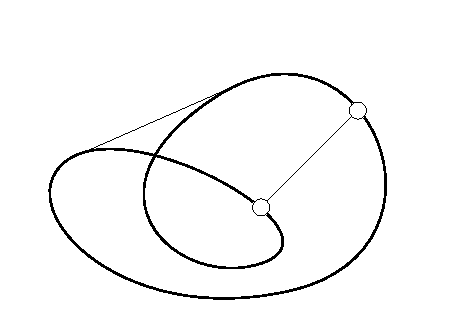
\includegraphics[scale=1,page=1]{mebius.pdf}} };
\end{tikzpicture}

\newpage
\begin{example} ($S^3$ $\mathbb{C}$  Hopf Fiber).
$S^3$ Fibration was peeoneered by Guillaume Brunerie.
\begin{lstlisting}
rot: (x : S1) -> Ξ S1 x x = split
    base -> loop1
    loop @ i -> constSquare S1 base loop1 @ i

mu : S1 -> equiv S1 S1 = split
    base -> idEquiv S1
    loop @ i -> equivPath S1 S1 (idEquiv S1)
                (idEquiv S1) (<j> \(x : S1) -> rot x @ j) @ i

H : S2 -> U = split
    north -> S1
    south -> S1
    merid x @ i -> ua S1 S1 (mu x) @ i

total : U = (c : S2) * H c
\end{lstlisting}
\end{example}

\begin{tikzpicture}
  \node[inner sep=20mm, fill=white, draw=black, line width=0.2mm] (img) at (0,0) {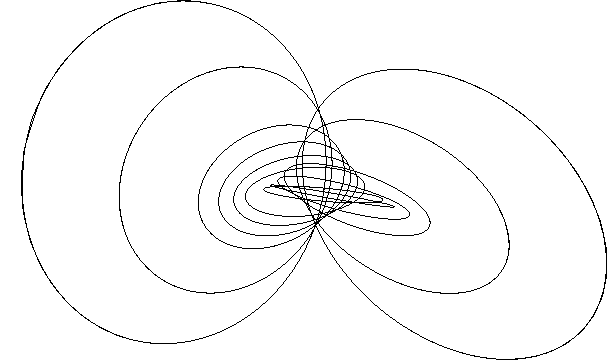
\includegraphics[scale=0.50,page=1]{hopf.pdf}};
\end{tikzpicture}

\begin{definition} (H-space).
H-space over a carrier $A$ is a tuple
$$
H_A=
\begin{cases}
A : U\\
e : A\\
\mu : A \rightarrow A \rightarrow A\\
\beta : \Pi (a:A), \mu(e,a)=a \times \mu(a,e)=a
\end{cases}
$$.
\end{definition}

\newpage
\begin{theorem} (Hopf Invariant).
Let $\phi: S^{2n-1} \rightarrow S^{n}$ a continuous map.
Then homotopy pushout (cofiber) of $\phi$ is
$cofib(\phi) = S^{n} \bigcup_\phi \mathbb{D}^{2n}$ has
ordinary cohomology
$$
H^{k}(\text{cofib}(\phi),\mathbb{Z})=
\begin{cases}
\mathbb{Z}\ for\ k=n,2n \\[2ex]
0\ otherwise
\end{cases}
$$
\end{theorem}


\begin{theorem} (Four).
There are fiber bundles:
$(S^0,S^1,p,S^1)$,
$(S^1,S^3,p,S^2)$,
$(S^3,S^7,p,S^4)$,
$(S^7,S^{15},p,S^8)$.
\end{theorem}

Hence for $\alpha,\beta$ generators of the cohomology groups in
degree $n$ and $2n$, respectively, there exists an integer $h(\phi)$
that expresses the {\textbf{cup product}} square of $\alpha$
as a multiple of $\beta$ --- $\alpha\sqcup\alpha=h(\phi)\cdot\beta$.
This integer $h(\phi)$ is called Hopf invariant of $\phi$.

\begin{theorem} (Adams, Atiyah).
Hopf Fibrations are only maps that have Hopf invariant $1$.
\end{theorem}


\bibliographystyle{plain}
\bibliography{hott}

\end{document}

